\begin{abstract}
In this document, we will mainly discuss the requirements for our image inpainting software.
We discuss both the functional and non-functional requirements as well as a specific hardware and software environment requirement and other necessary parts for our image inpainting ysstem.
\end{abstract}

\section{Requirement Analysis}
\subsection{Introduction to requirement analysis}
As Wikipedia says: in software engineering, requirements analysis encompasses those tasks that go into determining the needs or conditions to meet for a new or altered product or project, taking account of the possibly conflicting requirements of the various stakeholders, analyzing, documenting, validating and managing software or system requirements.

Thus requirement analysis is critical to the success of our image inpainting software. Also, the requirements should be well documented, actionable, measurable, traceable, and defined in detail.

In this following sections, we will discuss the requirements of this image inpainting software.

\subsection{System Overview}
\subsubsection{Definitions}
First, we should give a definition of image inpainting and this is a first solid step to the success of our image inpainting software.

Most of you will have some old damaged photos at your home with some black or gray spots on it. It is really a real-world requirement to fix that image in an acceptable way. We can't simply erase them in a single color because it will simply replace the damaged region which is useless. In these cases, a technique called image inpainting is used. Look at the image bellow:
\begin{figure}[H]
\centering
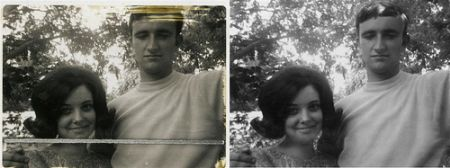
\includegraphics[width=9cm]{def.jpg}
\caption{An example of image inpainting}
\end{figure}
We can see that the left picture is damaged and
we want to fix those damaged regions. The right-hand-side picture is the in painted image, which is what we desire to get.

\subsubsection{History of image inpainting}
Inpainting, the technique of modifying an image in an undetectable form, is as ancient as art itself. Actually there are many professional image restorers in museums of ancient arts. Though the history of image restoration is quite long, computer-aided image inpainting appears quite late.

To our surprise, research on image inpainting emerged very late. In SIGGRAPH 2000 \cite{siggraph00}, Bertalmio proposed an algorithm to inpaint a image: after the user selects the regions to be
restored, the algorithm automatically fills in these regions with information surrounding them. The fill-in is done in such a way that
isophote lines arriving at the regions’ boundaries are completed inside.

Roth and Black \cite{cvpr05} later come up with a more general framework 
called \emph{Field of Experts} which is a Markov random field model. This
work relies on the result of Hinton \cite{neco02}, where Hinton discovers
that a factor in MRF can be modeled by a field of ``expert'' distributions.
In this work, they first learn the model and then apply the learned model
to Bertalmio's propagation method. Although this work in some sense captures
image structure, the blurring problem is also serious after our experiment.

Another different way to tackle this problem is proposed by Criminisi et al.\ 
 \cite{cvpr03,tip04}. They note that exemplar-based texture synthesis
 contains the essential process requred to replicate the structure of image.
 They introduce a priority for each exemplar and propagate according to
 the priority of each exemplar. This technique does not have the problem
 of blurring and can restore texture well, but may still fail for large
 object removal.

All these previous works shows that image inpainting is actually a really challenging job and to the best of our knowledge, there haven't been any practical software for image inpainting on market. Thus we will work hard on this project and finally open source this work on web so that other people can make use of it.

\subsection{Detailed system requirements}
\subsubsection{Computation platforms}
The recommended computation platform is shown as follows:
\begin{table}[H]
\centering
\begin{tabular}{|c|c|}
\hline
Hardware & Requirement \\ \hline
CPU & Intel Core i5 2GHz \\ \hline
Memory & 1GB \\ \hline
Disk & 100MB \\ \hline
GPU & N.A. \\ \hline
\end{tabular}
\caption{Hardware requirement spec}
\end{table}
Since to train the MRF model is CPU bound, we need the CPU to be at least Intel Core i5, which has a typical 2 GHz frequency. Also, our model is not typically designed for GPU and thus there is no limitation to GPU. For memory, the computation of MRF model requires much matrix computation and thus a 1GB memory is required. At last, we need to store the Berkeley image inpainting database, which contains 300 inpainted images and 100MB disk storage is required.
\subsubsection{Runtime environment requirement}
We want our image inpainting software to work cross-platform, thus a Windows OS or Linux OS will make sense. An example OS is shown in the following figure:
\begin{figure}[H]
\centering
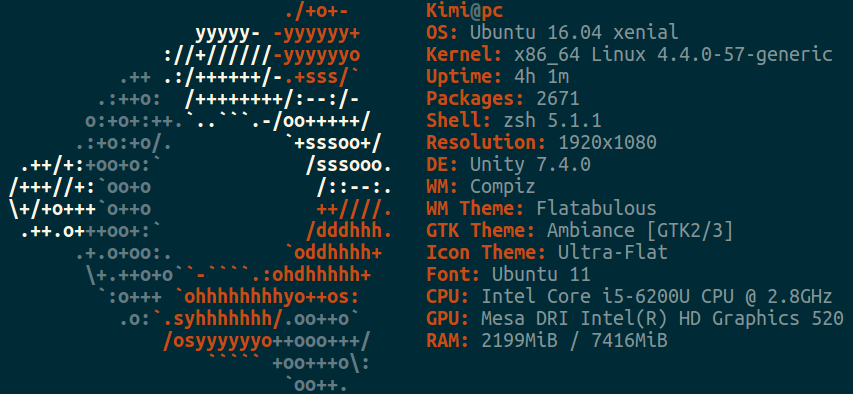
\includegraphics[width=8cm]{ubuntu.png}
\caption{Example operating system specification}
\end{figure}

As regard to programming language environment, we need a minimal MATLAB 2014 version in order to run our code in Windows OS. We recommend you use Python 2.7 instead of Python 3 since the libraries we use might not work fine with Python 3. Also, if you are using Linux, please make sure you have installed some cross-platform libraries such is python-tkinter so that our code can work
properly.

\subsection{Software Architecture requirements}
Software architecture is the  the fundamental structures of a software system, the discipline of creating such structures, and the documentation of these structures. Software architecture is so important that it may influence our development in all aspects.

We design the architecture of our image inpainting software to be a branch architecture. On the one hand, we implement a exemplar-based algorithm, which works fine for those images which explicit texture feature; on the other hand, we implement a MRF-based algorithm, which is based on probabilistic graphical model and works better for small damage inpainting. To combine these two components together, we have a unified user interface and it is easy for users to operate.

\subsection{Requirement analysis models}
\subsubsection{Functional requirements}
In this section, we will talk about the requirement of a real-world user. What's the requirements of a user to easily inpaint a image? We will list the requirements as follows:
\begin{itemize}
\item Input image: first, the user need to specify which image he/she is going to inpaint. In this case, the requirement is that we should provide a extra window to help the user browse in the file system to find the picture to be inpainted.
\item Input mask: similarly, the user also need to specify the input mask so that our image inpainting software can know which part it need to inpaint.
\item Inpainting progress: since image inpainting is not such an easy task, it may take minutes or even hours to finish inpainting a single image. Thus we provide the user with a window showing the progress of computation. This is a diagram that shows the convergence of our model, once the value of RGB channels all comes below 1, the image inpainting is finished.
\item Inpainting result: once the task of image inpainting is finished, a window will display both the original image and the inpainted version. Also, we will save the inpainted image to local file system so that user can further take the inpainted image for future use.
\item Error recovery: our model might not work for all images, in case our model does not fit well with the image given by user, we provide the user with an amount describing how ``good'' our model performs on this image and it is up to the user himself whether to proceed to inpaint this image.
\end{itemize}
\subsubsection{Non-functional requirements}
Non-functional requirements can vary from software to software, we will only list some of the key non-functional requirements for our image inpainting software:
\begin{itemize}
\item Platform compatibility: our image inpainting software works well both on Windows OS and Linux, which are two major operating systems in use.
\item Open source: since this is a course project and we do not want earn money from it, we will open source this project on GitHub.
\item Maintainability: this project is highly modularized and we believe the code will be easy for other community contributors to read and modify.
\item Response time: the execution time to inpaint an image may take 30 seconds to several minutes depending on the size to be inpainted. However, we believe our model works better than most of existing ones.
\item Documentation: we mainly provide 4 documentation:
\begin{enumerate*}
\item this report talks the design of this image inpainting software in detail;
\item a README file to instruct developers explore in this project;
\item a user guide for users who might not have a computer vision background;
\item a paper discussing the contribution of our work for those computer vision enthusiasts.
\end{enumerate*}
\end{itemize}
\subsubsection{Domain requirements}
We think the image inpainting software may apply to many different domains. We come up with some domains but applications should include but not restricted to these:
\begin{itemize}
\item Image restoration in museums of ancient arts
\item Help police recover damaged images
\item Help artists to remove texts from a image
\item Help people fix damaged old family photographs
\end{itemize}